\subsection{Simulation Results}
The simulation results for the $NO_x$ reduction prediction per time step for all the tests are plotted below.

\begin{figure}[H]
        \begin{minipage}{0.49\textwidth}
                \begin{figure}[H]
                        \centering
                        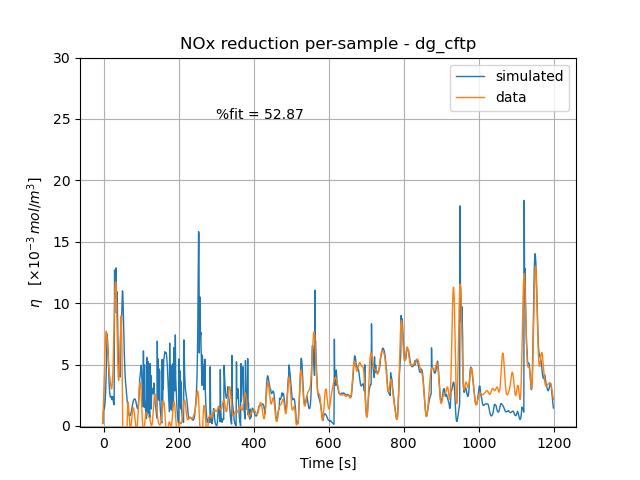
\includegraphics[width=\textwidth]{figs/15_figs/eta_sim_dg_cftp.png}
                \end{figure}
        \end{minipage}
        \begin{minipage}{0.49\textwidth}
                \begin{figure}[H]
                        \centering
                        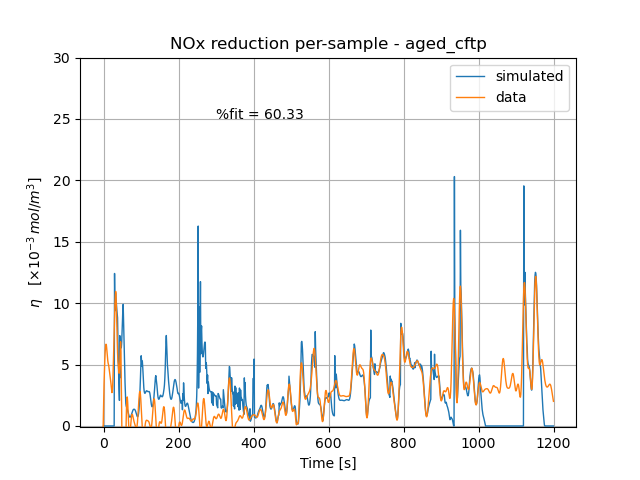
\includegraphics[width=\textwidth]{figs/15_figs/eta_sim_aged_cftp.png}
                \end{figure}
        \end{minipage}
        \caption{System response for cold FTP data}
\end{figure}

\begin{figure}[H]
        \begin{minipage}{0.49\textwidth}
                \begin{figure}[H]
                        \centering
                        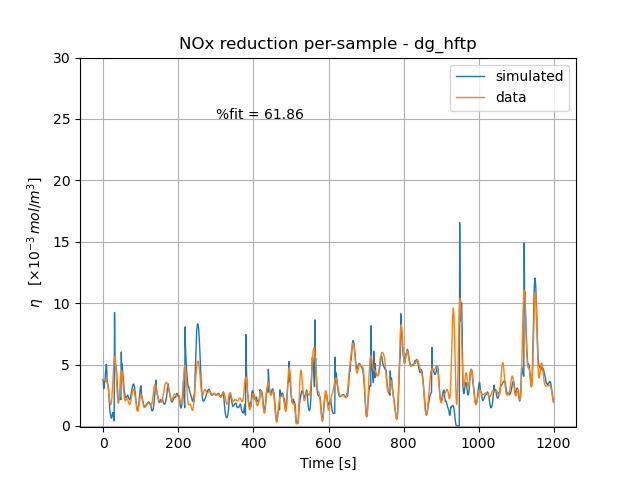
\includegraphics[width=\textwidth]{figs/15_figs/eta_sim_dg_hftp.png}
                \end{figure}
        \end{minipage}
        \begin{minipage}{0.49\textwidth}
                \begin{figure}[H]
                        \centering
                        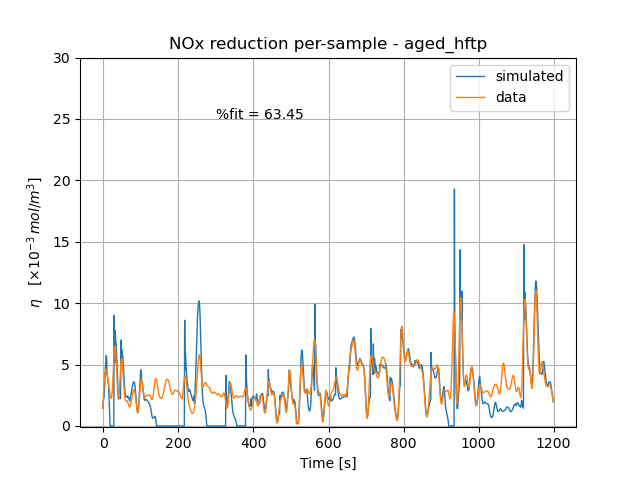
\includegraphics[width=\textwidth]{figs/15_figs/eta_sim_aged_hftp.png}
                \end{figure}
        \end{minipage}
        \caption{System response for hot FTP data}
\end{figure}

\begin{figure}[H]
        \begin{minipage}{0.49\textwidth}
                \begin{figure}[H]
                        \centering
                        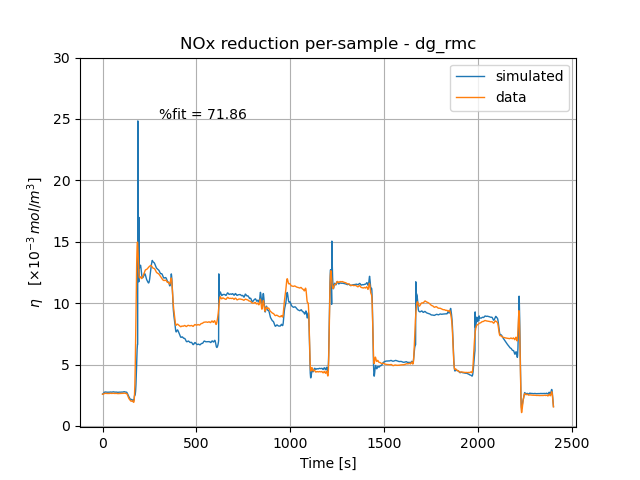
\includegraphics[width=\textwidth]{figs/15_figs/eta_sim_dg_rmc.png}
                \end{figure}
        \end{minipage}
        \begin{minipage}{0.49\textwidth}
                \begin{figure}[H]
                        \centering
                        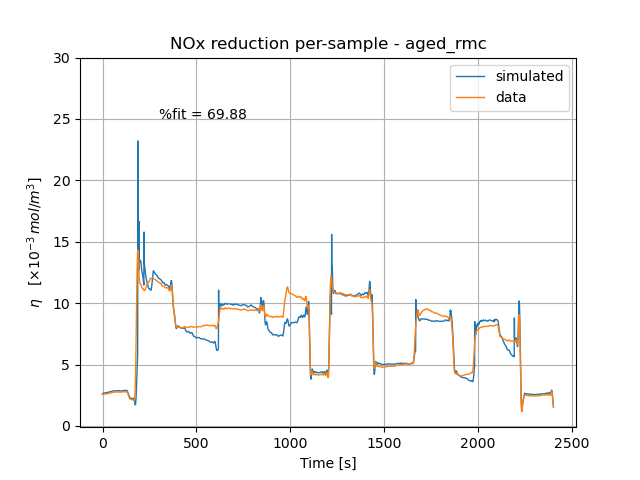
\includegraphics[width=\textwidth]{figs/15_figs/eta_sim_aged_rmc.png}
                \end{figure}
        \end{minipage}
        \caption{System response for RMC data}
\end{figure}


\begin{table}[H]
        \centering
        \caption{$\%$fit of the models with test data}
        \begin{tabular}{l l c c}
                \hline \hline
                Age & Test & Hybrid Nonlinear Model & Linearized CSTR Model \\ \hline \hline
                Degreened & RMC & 71.86 & 19.98 \\
                Aged      & RMC & 69.88 & 27.66 \\ \hline
                % =========================================
                Degreened & hot FTP & 61.86 & 7.10 \\
                Aged      & hot FTP & 63.45 & 7.38 \\ \hline
                % =========================================
                Degreened & Cold FTP & 52.87 & 23.24 \\
                Aged      & Cold FTP & 60.33 & 23.19 \\ \hline
                \hline
        \end{tabular}

        $\%fit = 100 \times \lr{1 - \frac{\norm{Y- \hat Y}}{\norm{Y -
        mean(Y)}}}$ \\
        $\%fit$ is the percentage of the measured output that was explained by the
        model.
\end{table}

Thus, the hybrid nonlinear model consistently fits the data with a goodness of fit value greater than $60\%$ for all the test-cases.
